
\section{Apêndice - Modelos Regressão linear, XGB Regressão, Ligth GBM Regressão e Regressão de Floresta Aleatória 18h a 21h}\label{sec:lrxgblgbmrf18}

\begin{figure}[H]
	\centering
	\caption{Comparação dos modelos Regressão linear, XGB Regressão, Ligth GBM Regressão e Regressão de Floresta Aleatória, 1 dia a frente }
	\label{fig:1-LR-XGB-LGBM-RF}
	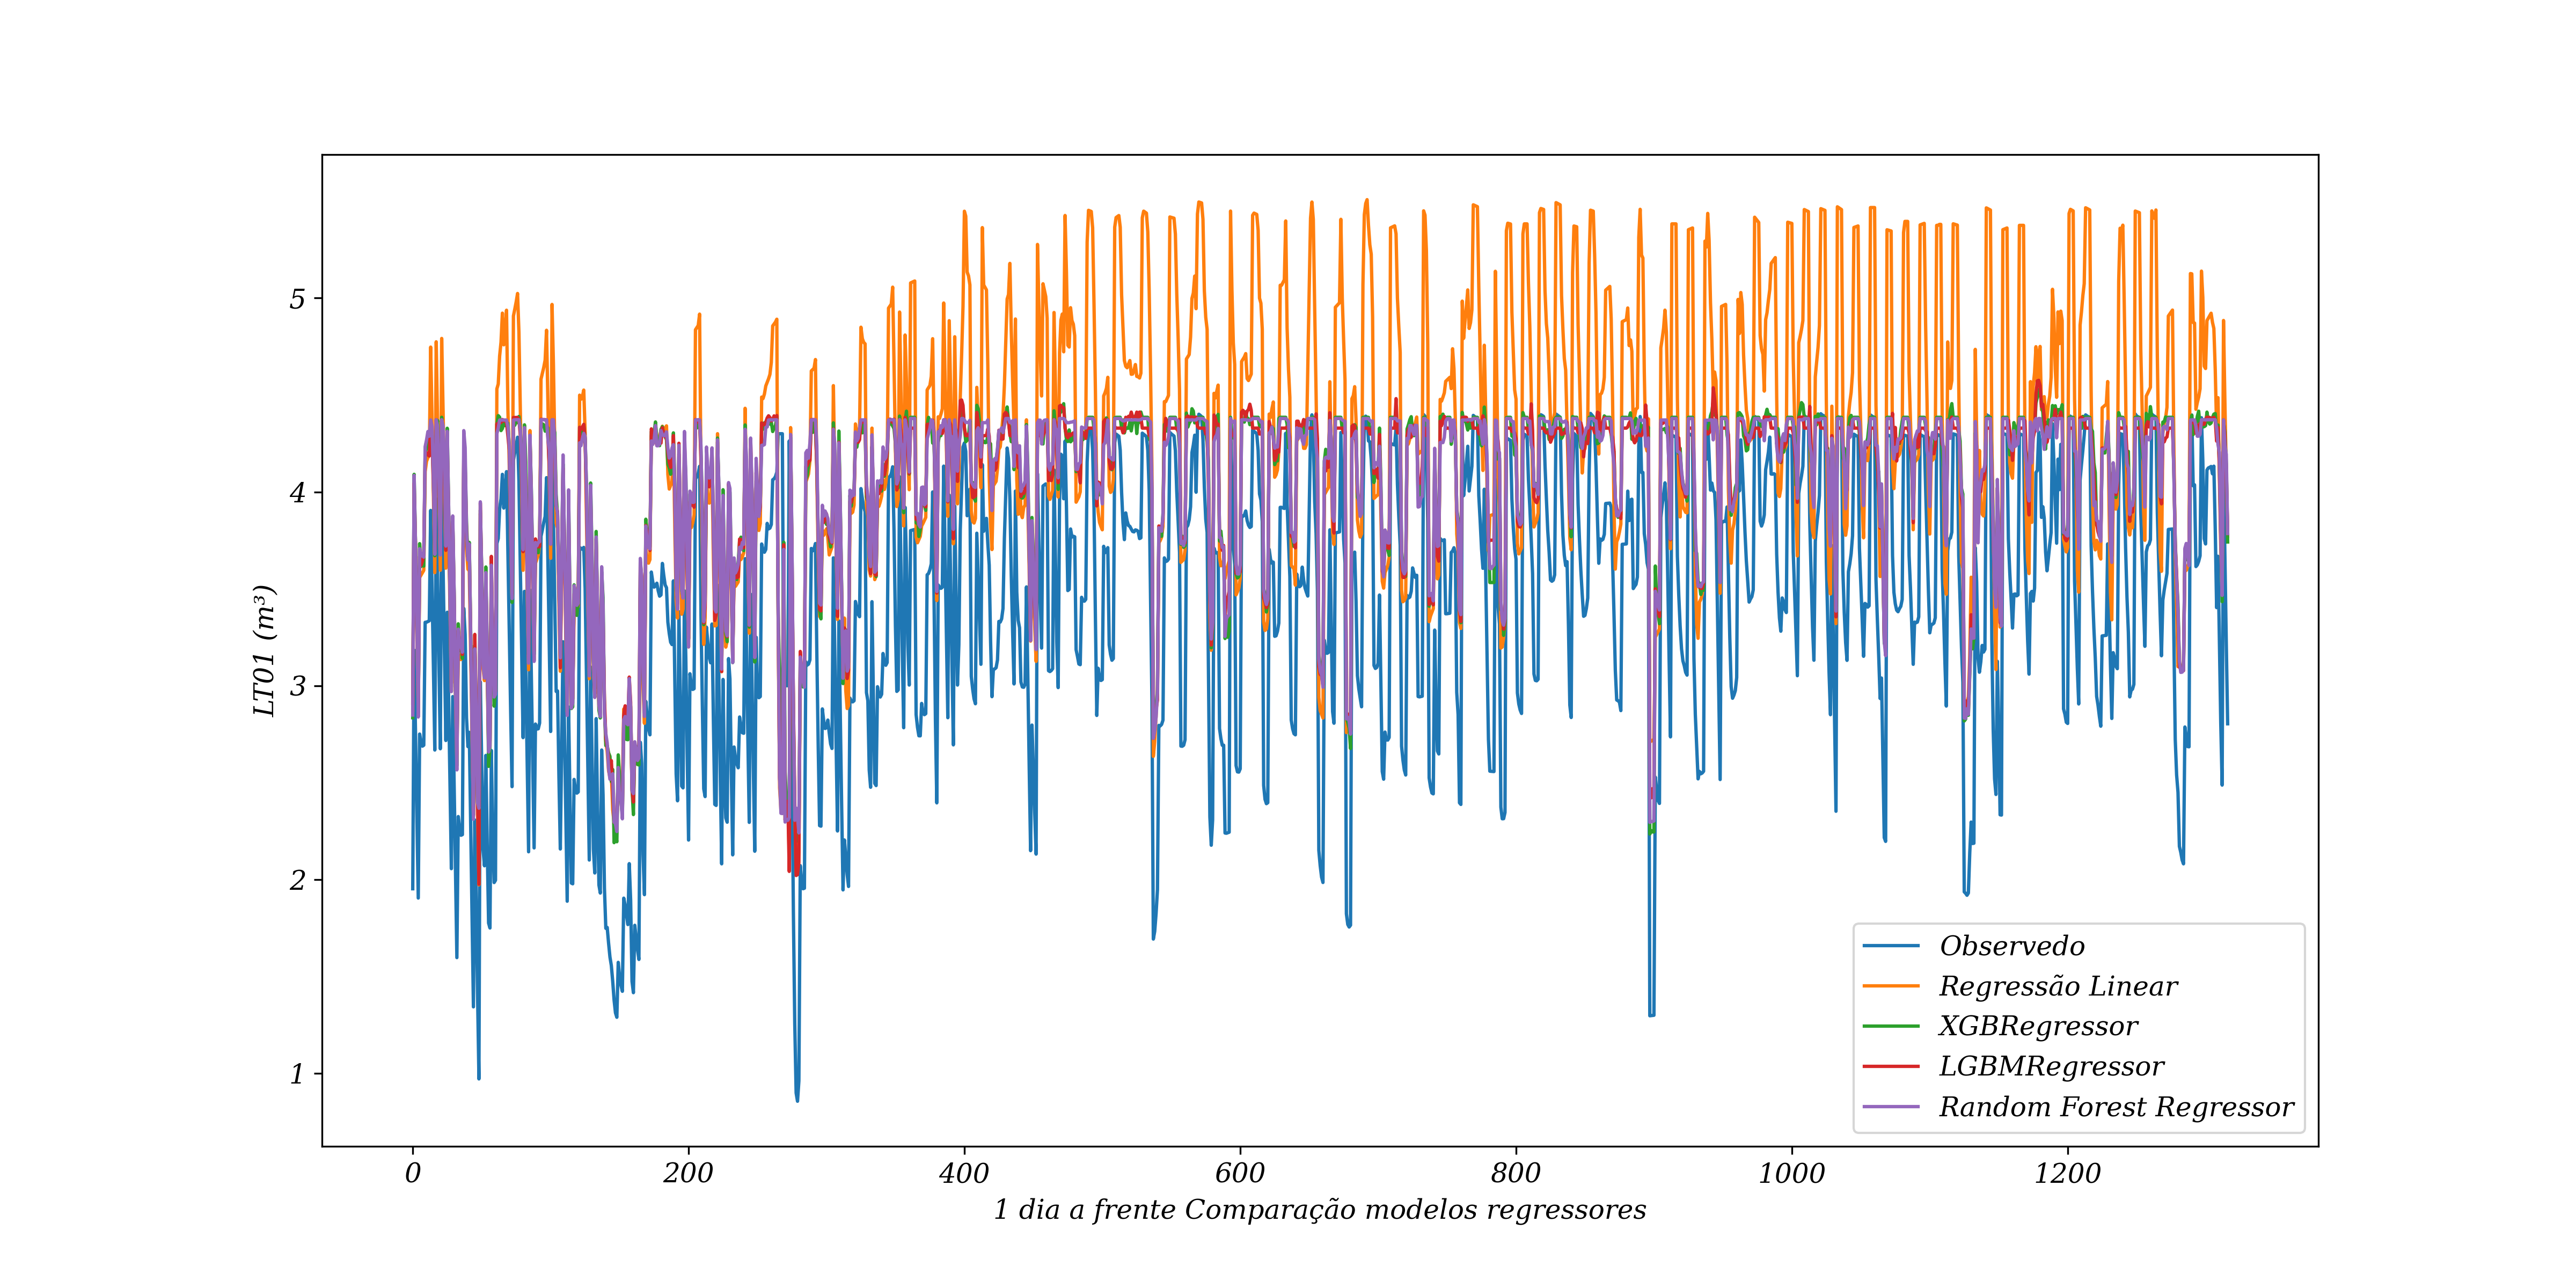
\includegraphics[width=1\linewidth]{Apendices/Figuras/modelagem-18-a-21h/1-LR-XGB-LGBM-RF}
	
	Fonte: Autoria própria.
\end{figure}

\begin{figure}[H]
	\centering
	\caption{Comparação dos modelos Regressão linear, XGB Regressão, Ligth GBM Regressão e Regressão de Floresta Aleatória, 10 dias a frente }
	\label{fig:10-LR-XGB-LGBM-RF}
	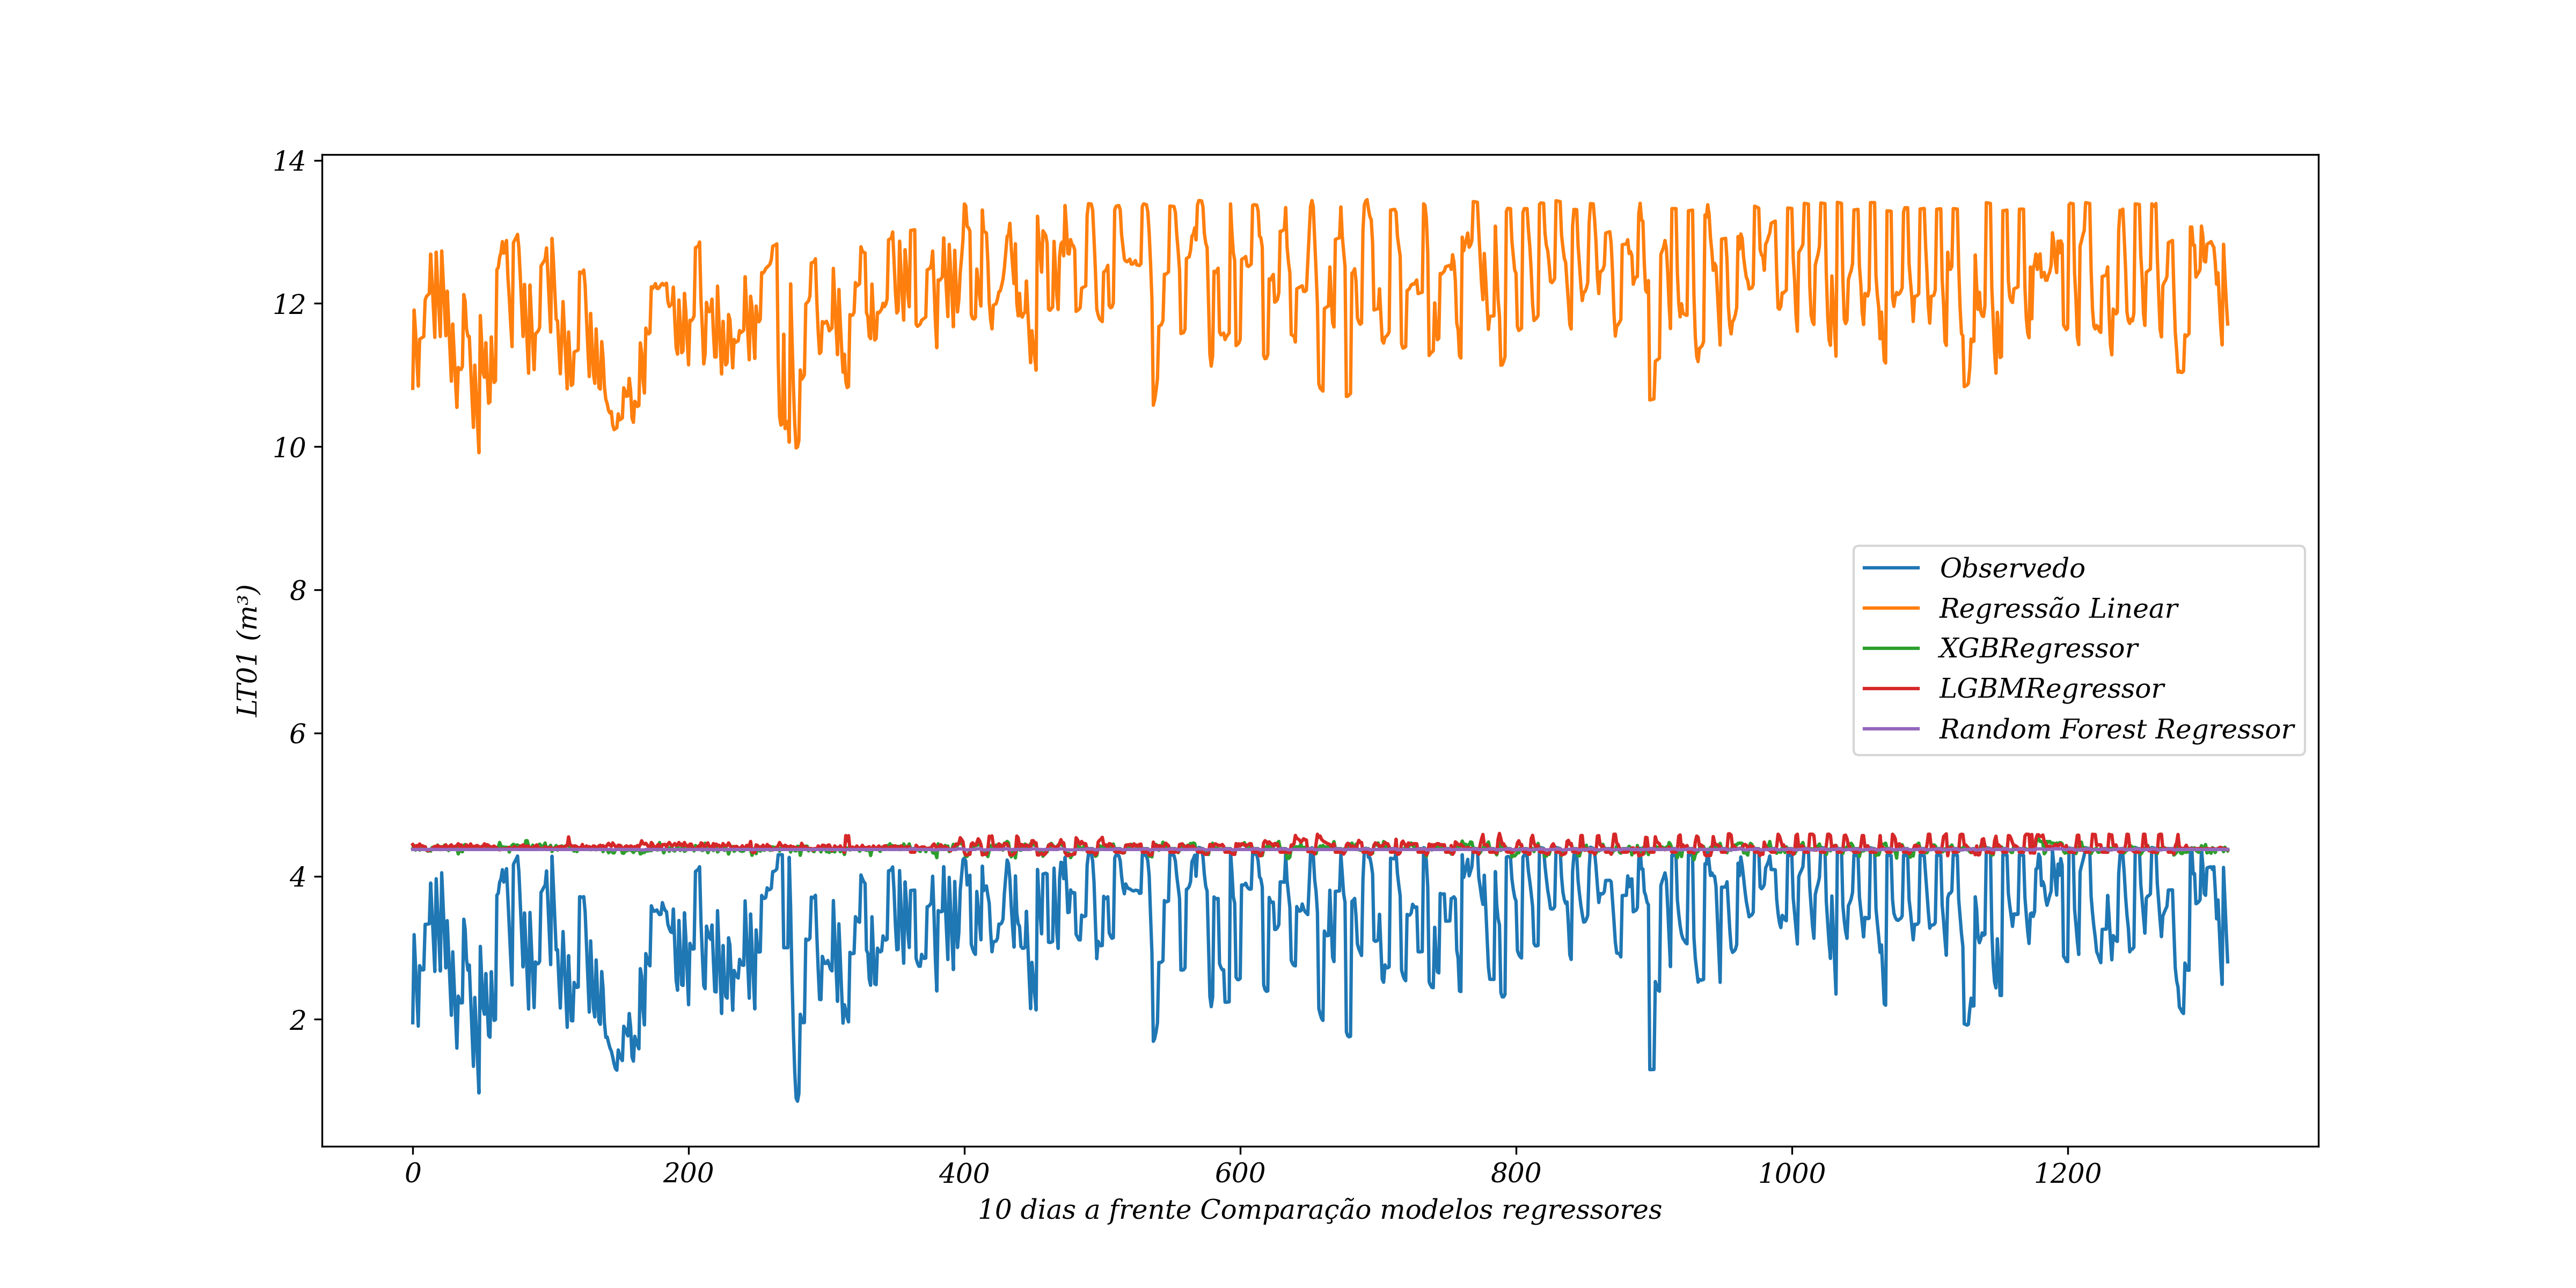
\includegraphics[width=1\linewidth]{Apendices/Figuras/modelagem-18-a-21h/10-LR-XGB-LGBM-RF}
	
	Fonte: Autoria própria.
\end{figure}


\begin{figure}[H]
	\centering
	\caption{Comparação dos modelos Regressão linear, XGB Regressão, Ligth GBM Regressão e Regressão de Floresta Aleatória, 30 dias a frente }
	\label{fig:30-LR-XGB-LGBM-RF}
	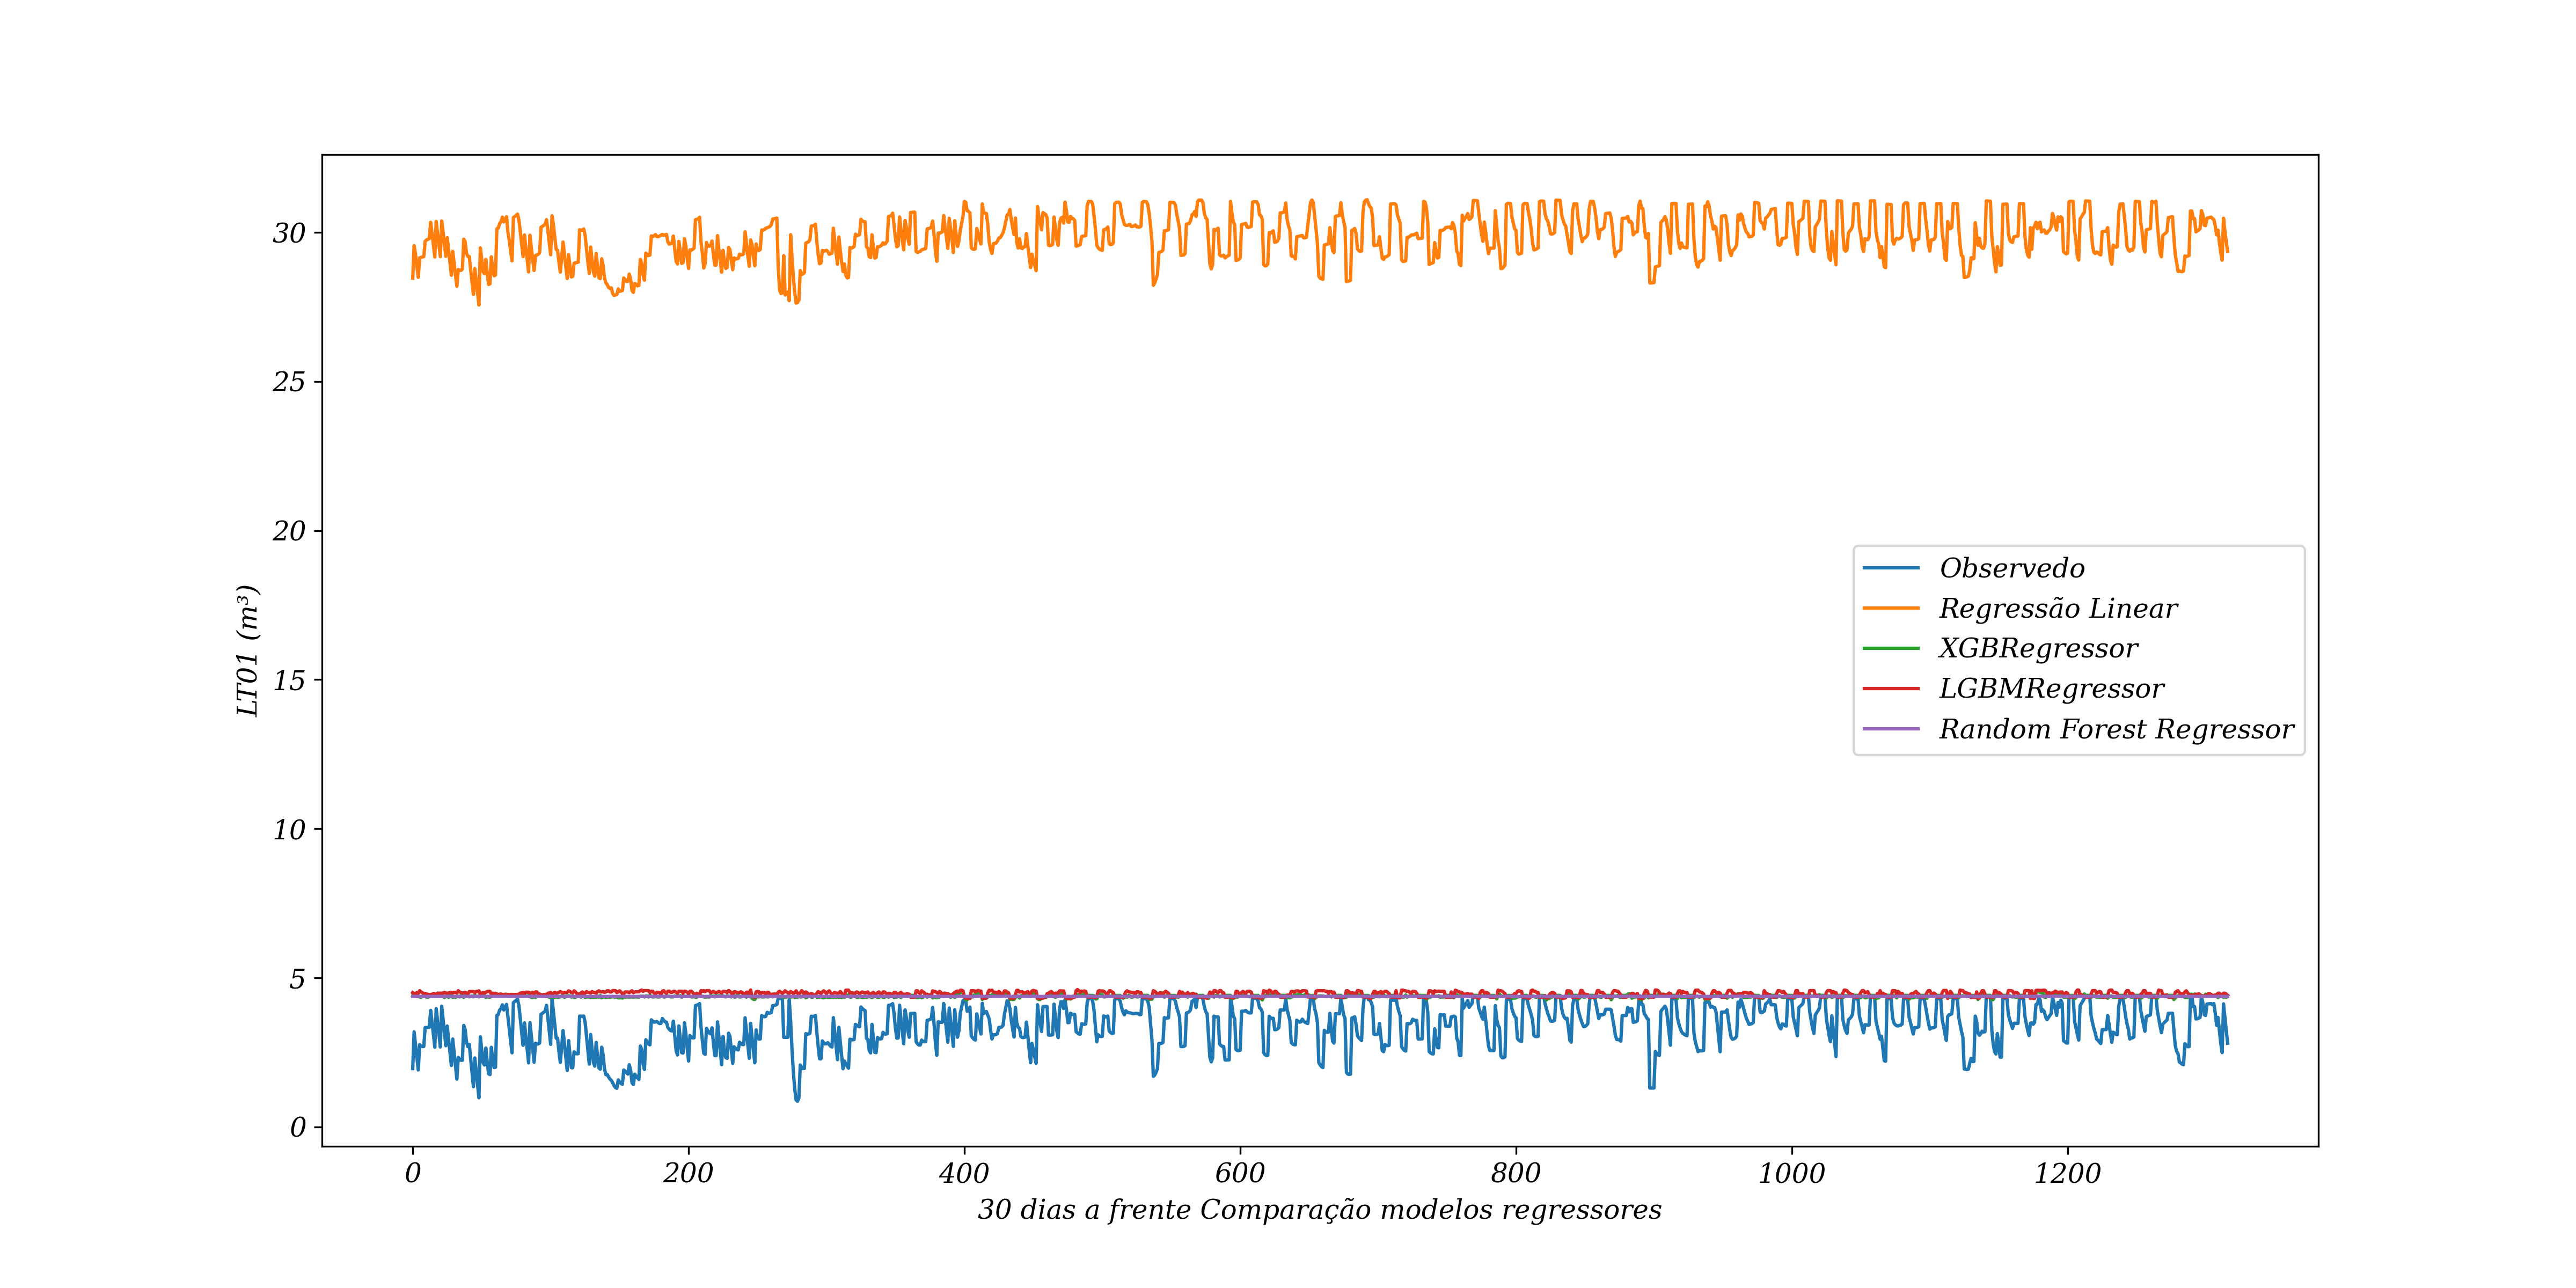
\includegraphics[width=1\linewidth]{Apendices/Figuras/modelagem-18-a-21h/30-LR-XGB-LGBM-RF}
	
	Fonte: Autoria própria.
\end{figure}

\begin{figure}[H]
	\centering
	\caption{Comparação dos modelos Regressão linear, XGB Regressão, Ligth GBM Regressão e Regressão de Floresta Aleatória, 60 dias a frente }
	\label{fig:60-LR-XGB-LGBM-RF}
	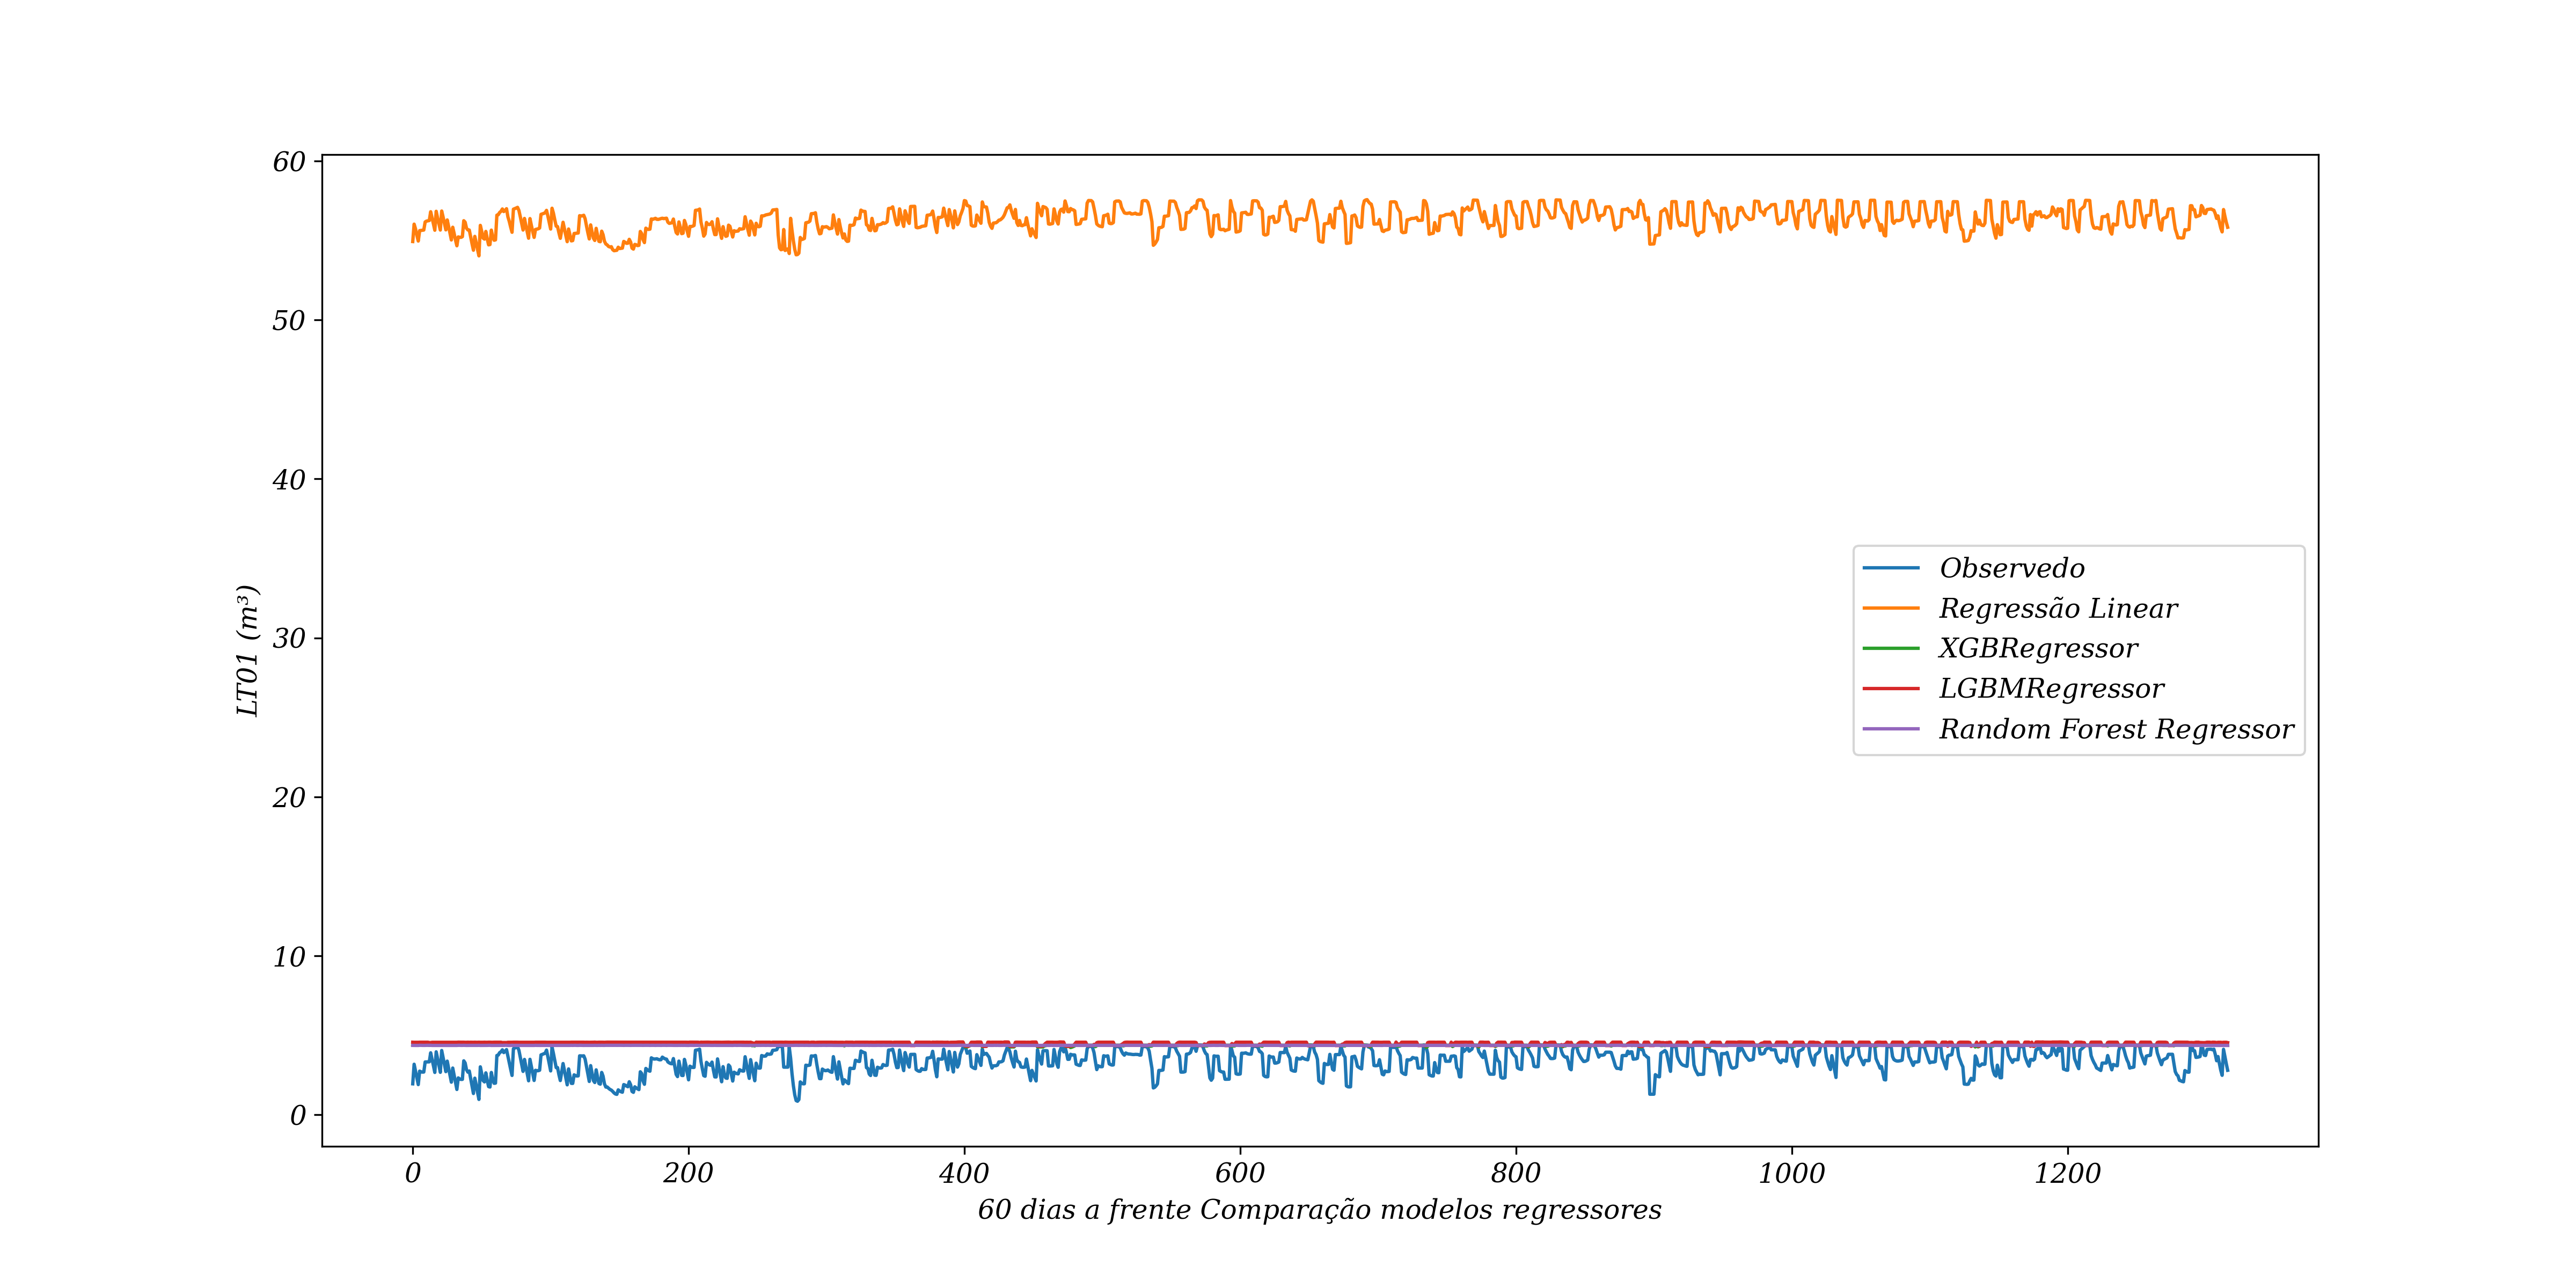
\includegraphics[width=1\linewidth]{Apendices/Figuras/modelagem-18-a-21h/60-LR-XGB-LGBM-RF}
	
	Fonte: Autoria própria.
\end{figure}